%
% CHAPTER 7.- Interesting Questions
%

%
%  Section 1
%    - (major) We have to clarify which description function we are using
%  Section 4
%    - (major) Missing reference to combined nescience proposition
%

\chapterimage{thinker.pdf}

\chapter{Interesting Questions}
\label{chap:Interesting-Research-Questions}

\begin{quote}
\begin{flushright}
\emph{It is not the answer that enlightens,\\
but the question. \\}
Eugène Ionesco
\end{flushright}
\end{quote}
\bigskip

In this chapter, we propose a set of metrics for classifying research topics based on their potential as a source of interesting problems, along with a methodology for assisted discovery of new questions. The methodology can be used to identify new applications of existing tools to solve open problems and to discover new, previously unexplored research topics. The methodology is applicable to both intradisciplinary and interdisciplinary topics, but the most interesting outcomes are obtained in the latter case. In Chapters \ref{chap:philosophy-science} and \ref{chap:computational-creativity}, we demonstrate the application of the methodology in practice and suggest new questions and research topics.

Our primary assumption is that a research question is interesting if it meets the following three criteria\index{Criteria for Interesting Questions}:

\bigskip

\begin{description}
\item[C1] The question should be new and original, meaning that it has not been previously considered.
\item[C2] Upon its resolution, there should be a significant increase in our knowledge about one or more specific research topics.
\item[C3] It should have practical applications that could have a substantial (hopefully positive) impact on people's lives.
\end{description}

\bigskip

Some researchers may argue that the requirements presented may not be the most suitable. For instance, researchers from the so-called "hard sciences", such as pure mathematics and theoretical physics, might object that practical applications are not a crucial factor in pursuing an interesting open problem. In such situations, the metrics introduced can be redefined since they are simply mathematical abstractions, and the same methods can still be applied. The methodology described is universal and can be employed in various domains, not only in discovering new research questions. In fact, the metrics and methods outlined can be utilized in any field where there is a vast collection of interconnected describable objects, and the objective is to uncover new and previously unknown objects. The precise definition of concepts like relevance graph, applicability graph, or maturity will be contingent on the field in which the approach is being employed. Nevertheless, as in the case of Chapter \ref{chap:Nescience}, we prefer to present the methodology and new concepts in the specific context of scientific research because it aids in their comprehension.

It is worth mentioning the relationship between this new methodology and the areas of computational creativity and artificial intelligence. What is proposed in this chapter is an algebraic approach to the assisted discovery of potentially interesting questions. The intention is not for the computer to understand the meaning of the questions posed. Furthermore, not all the questions generated are necessarily relevant or even meaningful. It is the responsibility of the researchers to assess the proposed combinations of topics and determine if any of the questions are appropriate.

We have already explored two dimensions for classifying topics: miscoding (Chapter \ref{chap:Miscoding}) and mismodel (Chapter \ref{chap:Redundancy}). These metrics enable us to quantitatively assess our understanding of a topic, which we refer to as nescience. According to criterion \textbf{C2} of our list of requirements for questions, the higher the nescience of a topic, the greater its potential as a source of interesting research questions. In this section, we will introduce two additional metrics for characterizing topics: relevance and applicability. Relevance measures the impact a topic has on people's lives and serves as a complement to nescience. Applicability measures how frequently a topic has been applied in other areas and enables us to identify new applications of already existing technologies.

%
% Section: Relevance
%

\section{Relevance}

Before to measure relevance of a topic, that is, its impact in people's life, we have to introduce the concept of \emph{relevance graph}\index{Relevance graph}. The relevance graph is a graph that describes which people is affected by which research topics.

\begin{definition}\index{Relevance Graph}
\label{def:relevance-graph}
We define the \emph{relevance graph}, denoted by $\mathbf{RG}$, as the bipartite graph $\mathbf{RG} = (\mathcal{T}, \mathcal{P}, E)$, where $\mathcal{T}$ is the set of topics, $\mathcal{P}$ the set of people, and $E\subseteq\left\{ \left(i,j\right):i\in \mathcal{T},j\in \mathcal{P} \right\}$ is the set of arcs between topics and people. An arc $(i, j)$ belong to $E$ if, and only if, person $j$ is affected by topic $i$.
\end{definition}

When we refer to the set of people $\mathcal{P}$, we are referring to all individuals in the world. An edge in the relevance graph indicates that someone is affected by a topic, rather than being interested in it. The exact meaning of "being affected by" is a difficult to define concept that is beyond the scope of this book. Therefore, our definition of the relevance graph is a mathematical abstraction. In Section \ref{sec:Classification_Research_Topics}, we will explore how to approximate this quantity in the case of scientific research topics. In Chapter \ref{chap:Software-Engineering}, we will provide an alternative interpretation of the relevance graph in the context of measuring software quality.

\begin{example}
A man who is affected by ALS (amyotrophic lateral sclerosis) disease will be connected to the ALS topic in the graph. His spouse will also be connected because she is likely to be impacted by the consequences of the disease as well. However, a researcher who is interested in ALS as a research problem, rather than someone suffering the disease, will not be connected to the ALS node in the graph.
\end{example}

Optionally, we can add a weight $w_{ij}\in\left[0,1\right]$ to the edges of the graph to specify the degree in which a person $j$ is affected by a topic $i$. A weight of $1$ could represent a life-or-death dependence, and $0$ would mean that this person is not affected at all. In Figure \ref{fig:Relevance-Graph} it is depicted an example of relevance graph. 

\begin{figure}[h]
\centering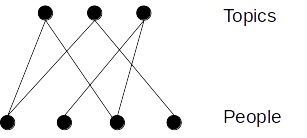
\includegraphics[scale=0.7]{bipartite_graph}
\caption{\label{fig:Relevance-Graph}Relevance Graph}
\end{figure}

\begin{definition}\index{Relevance}
\label{def:relevance}
We define the \emph{relevance} of a topic $t \in \mathcal{T}$, denoted by $R(t)$, as the degree of the node $t$ in the relevance graph, that is, $R(t) = deg(t)$.
\end{definition}

Intuitively, the higher the relevance of a topic, the higher its potential as a source of interesting questions, since we will be working on a problem that affects many people.

Sometimes it is covenient to work with a normalized version of the relevance of a topic.

\begin{definition}\index{Normalized relevance}
\label{def:normalized_relevance}
We define the \emph{normalized relevance} of a topic $t \in \mathcal{T}$, denoted by $\bar{R}(t)$, as the normalized degree of the node $t$ in the relevance graph, that is, $\bar{R}(t) = deg(t) / d(E)$.
\end{definition}

We could have computed also $deg(p)$, that is, the number of edges that links to a person $p$ in the relevance graph, as a measure of the number of topics that affects a particular person. However, this quantity is not used in the theory of nescience. The relation between $deg(t)$ and $deg(p)$ is given by the degree sum formula:
\[
\sum_{t \in \mathcal{T}} deg(t) = \sum_{p \in \mathcal{P}} deg(p) = d(E)
\]

Next proposition proves that adding more topics to a research project can only increase its relevance. Of course, a research project dealing with "life, the universe and everything" would be a highly relevant one, but very impractical as well. How to properly combine research topics will be described in Section \ref{sec:New_Research_Topics}.

\begin{proposition}
\label{prop:nondecreasing_relevance}
Given any two topics $t_{1}, t_{2} \in \mathcal{T}$, we have that $R(t_{1}) + R(t_{2}) \geq R(t_{1})$.
\end{proposition}
\begin{proof}
Let $S_{1}$ the set of people connected to to topic $t_{1}$ in the relevance graph, and  $S_{2}$ the set of people connected to to topic $t_{2}$. Since $d \left( S_{1} \cup S_{2} \right) = d(S_{1}) + d(S_{2}) - d(S_{1} \cap S_{2})$, and $d(S_{2}) - d(S_{1} \cap S_{2}) \geq 0$ we have that $d \left( S_{1} \cup S_{2} \right) \geq d(S_{1})$ and thus $R(t_{1}) + R(t_{2}) \geq R(t_{1})$.
\end{proof} 

Finally, we define the concept of interestingness of a topic as a source of interesting problems, that is, how likely is that the topic can be used in a new interesting research question, as a function of its nescience and relevance. We can visualize topics in a two-dimensional vector space, in which one dimension is nescience, and the other one is relevance. In this interpretation, a natural choice of interestingness function would be the euclidean distance from the origin.

\begin{definition}\index{Interestingness of a topic as a problem}
Given a topic $t \in \mathcal{T}$, we define the \emph{interestingness of the topic as a problem}, denoted by $IP(t)$, as:
\[
IP(t) = \sqrt{ \nu(t)^2 +  R(t)^2 }
\]
\end{definition}

Intuitively, a topic is interesting as a problem worth investigating if it has a large relevance (it has high impact in people's life) and a large nescience (it is not very well understood). In this sense, we are borrowing ideas from Popper's falsificationism: the more risky is a conjecture, the higher the advance achieved in science given its confirmation.

\begin{example}
\label{ex:fixed_point}
The fixed point theorem has some relevance, since people life's can be indirectly affected by its implications, but since it is a very well understood theorem (our nescience is very low), it is not a very interesting research problem by itself.

World War I is a very relevant topic, because it had a huge impact on many people's life, and also it is not very well understood topic, since it takes hundreds of pages to explain its causes, and there is no general agreement among the specialists. So, according to our definition, it is a very interesting research problem.
\end{example}

In practice, it is convenient to work with the normalized version of the relevance metric, so that we can avoid the case that our questions are always related to a small subset of extremely interesting topics.
\[
IP(t) = \sqrt{ \nu(t)^2 +  \bar{R}(t)^2 }
\]

%
% Applicability
%

\section{Applicability}

As mentioned in Example \ref{ex:fixed_point}, the fixed point theorem is not particularly compelling as a research problem on its own. However, it is an essential mathematical result since it has broad applications in proving many other theorems. In this section, we introduce the concept of \emph{applicability}, which is a novel measure enabling us to identify which topics are important since they can serve as as tools for understanding other topics. From a mathematical point of view, we say that a tool can be applied to a topic if the conditional nescience (see Section \ref{sec:conditional_nescience}) of the topic given the tool is smaller that the unconditionall nescience of the topic.

Before to formally define the concept of applicability, first we have to introduce a new bipartite graph that describes which topics has been applied as tools to other topics.

\begin{definition}\index{Applicability graph}
\label{def:applicability-graph}
We define the \emph{applicability graph}, denoted by $AG$, as the directed graph $AG = (\mathcal{T}, E)$, where $\mathcal{T}$ is the set of research topics, and $E\subseteq\left\{ (i,j):i,j\in \mathcal{T} \right\} $. An arc $(i, j)$ belong to $E$ if $N \left( t_i \mid t_j \right) < N \left( t_i \right)$. The weight of the arc $(i, j)$ is given by $w_{ij} = N \left( t_i \right) - N \left( t_i \mid t_j \right)$.
\end{definition}

The applicability graph helps us identify those topics that can be pontentially used as tools to understand other topics. The following defintion formally introduces this idea.

\begin{definition}\index{Applicability}
\label{def:applicability}
Given the applicability graph $AG = (\mathcal{T}, E)$, the \emph{applicability} of a topic $t_i \in \mathcal{T}$, denoted by $A(t_i)$, is defined as the sum of the weights of the arcs in the outdegree of $t_i$, that is:
\[
A(t_i) = \sum_{(i, j) \in E} w_{ij}
\]
where $E$ is the set of arcs in the applicability graph, and $w_{ij}$ is the weight of the arc $(i, j)$.
\end{definition}

A topic with higher applicability will have a greater overall impact on the understanding of other topics, and intuitively, the higher the applicability of a topic, the higher its potential as a tool that can be applied to solve open problems. If a tool has been successfully applied multiple times in the past to address open problems, it is more likely that it can be effectively used to solve other open problems as well.

Next proposition proves that the combination of two topics can only increase their applicability. That is, the more tools we have at our disposal, the more problems we could solve in principle.

\begin{proposition}
Given any two topics $t_1, t_2 \in \mathcal{T}$, we have that $A(t_1) + A(t_2) \geq A(t_1)$.
\end{proposition}
\begin{proof}
Use the same argument than in Proposition \ref{prop:nondecreasing_relevance}.
\end{proof}

In order to better compare the applicability of different topics and understand their relative importance in a standardized way, it is useful to introduce a normalized version of the applicability measure.

\begin{definition}\index{Normalized Aapplicability}
\label{def:normalized-applicability}
Given the applicability graph $AG = (\mathcal{T}, E)$, the \emph{normalized applicability} of a topic $t_i \in \mathcal{T}$, denoted by $A_n(t_i)$, is defined as the ratio of the applicability of $t_i$ to the maximum possible applicability value, expressed as:
\[
\tilde{A}(t_i) = \frac{A(t_i)}{\max_{t_k \in \mathcal{T}} A(t_k)}
\]
where $A(t_i)$ is the applicability of topic $t_i$ as defined in Definition \ref{def:applicability}, and $\max_{t_k \in \mathcal{T}} A(t_k)$ is the maximum applicability value among all topics in $\mathcal{T}$.
\end{definition}

Normalized applicability scales the original applicability value of a topic to a range between 0 and 1, allowing for easier comparison across different topics.

In practice, it is very difficult to compute the applicability graph, since for the majority of the topics, the quantity $N \left( t_i \mid t_j \right)$ has not been estimated. In order to solve this problem, we can use an approximation to the applicabilitiy graph, in which the arcs have no weight, and an edge $(i, j)$ represents that the topic $j$ has been applied to solve the problem $i$. For example, there would be a direct link between the topics "graph theory" and "recommendation engines", since graph theory has been successfully applied to the problem of how to recommend purchase items to customers over Internet.

\begin{definition}\index{Simplified applicability graph}
\label{def:simplified-applicability-graph}
We define the \emph{simplifiled applicability graph}, denoted by $SAG$, as the directed graph $SAG = (\mathcal{T}, E)$, where $\mathcal{T}$ is the set of research topics, and $E\subseteq\left\{ (i,j):i,j\in \mathcal{T} \right\} $. An arc $(i, j)$ belong to $E$ if the topic $j$ has been used to understand topic $i$.
\end{definition}

Using this simplified version of the applicability graph, the concept of applicability becomes:

\begin{definition}\index{Simplified applicability}
\label{def:simplified-applicability}
We define the \emph{simplified applicability} of a topic $t\in \mathcal{T}$, denoted by $SA(t)$, as the outdegree of that node in the applicability graph, that is:
\[
SA(t) = outdeg(t)
\]
\end{definition}

And the corresponding normalized version becomes:

\begin{definition}\index{Normalized simplified applicability}
\label{def:normalized-simplified-applicability}
Given the simplified applicability graph $SAG = (\mathcal{T}, E)$, the \emph{simplified normalized applicability} of a topic $t_i \in \mathcal{T}$, denoted by $SA_n(t_i)$, is defined as the ratio of the simplified applicability of $t_i$ to the maximum possible simplified applicability value, expressed as:
\[
SA_n(t_i) = \frac{SA(t_i)}{\max_{t_k \in \mathcal{T}} SA(t_k)}
\]
where $SA(t_i)$ is the simplified applicability of topic $t_i$ as defined in Definition \ref{def:applicability}, and $\max_{t_k \in \mathcal{T}} SA(t_k)$ is the maximum applicability value among all topics in $\mathcal{T}$.
\end{definition}

When using topics as tools, we are primarily interested in those topics that are better understood. Generally, relying on a background knowledge that is poorly understood is not advisable, even if it significantly reduces the (conditional) nescience of our problem. In the following definition, we will introduce the concept of the maturity of a topic as one minus its nescience.

\begin{definition}\index{Maturity}
Given a topic $t \in \mathcal{T}$, we define the \emph{maturity} of topic $t$, denoted as $M(t)$, as:
\[
M(t) = \nu(t)^{-1}
\]
\end{definition}

Intuitively, the more mature a topic is, the greater its utility in solving other open problems. Highly immature topics should not be applied as tools to address open problems, as doing so would merely transfer our lack of understanding from one topic to another.

\begin{example}
Linear regression is a highly mature topic, since its nescience is very small.
\end{example}

Finally, we define the concept of interestingness of a topic as a source of interesting tools, that is, how likely is that the topic can be used to solve a new problem, as a function of its maturity and applicability. Similar to the definition of relevance introduced in the previous section, topics can be visualized within a two-dimensional vector space, where one dimension represents maturity and the other represents applicability. The interestingness of a topic will be determined by its Euclidean distance from the origin.

\begin{definition}\index{Interestingness of a topic as a tool}
Given a topic $t \in \mathcal{T}$, we define the \emph{interestingness of the topic as a tool}, denoted by $IT(t)$, as:
\[
IT(t) = \sqrt{ M(t)^2 +  A(t)^2 }
\]
\end{definition}

Intuitively, a topic is considered interesting as a tool if it is thoroughly understood and has already been applied to numerous other problems.

\begin{example}
The Pythagorean theorem (in a right-angled triangle, the square of the length of the hypotenuse is equal to the sum of the squares of the other two sides) is undoubtedly one of the most widely used and applied theorems in various fields and practical situations, including but not limited to: engineering (calculating distances, angles, and forces in structures and mechanical systems), architecture (determining lengths and angles in building design and construction projects), land surveying (measuring distances and calculating areas of land parcels), physics (analyzing problems in mechanics, optics, and electromagnetism), computer graphics and game development (calculating distances and angles in 2D and 3D spaces) or trigonometry(serving as a foundation for the study of trigonometric functions and their applications). The widespread application of the Pythagorean theorem to so many fields is due to its simplicity and its ability to describe complex geometric relationships.
\end{example}


%
% Section: Interesting Questions
%

\section{Interesting Questions}

In the quest to uncover novel research questions, combining existing topics from various fields can yield fascinating results. By applying tools and methodologies from one topic to solve problems in another, researchers can explore innovative avenues and potentially make groundbreaking discoveries. In the following section, we delve into the methodology of combining topics to generate questions, along with the concept of interestingness and interdisciplinary research.

In our methdology, a interesting question emerges from the combination of two pre-existing topics. Given a pair of a topics in $t_1, t_2 \in \mathcal{T}$, the question can be framed as "\emph{can we apply the tool described by topic $t_1$ to solve the problem described by topic $t_2$?}".

\begin{definition}\index{Question}
Given two topics $t_1, t_2 \in \mathcal{T}$, a \emph{question}, denoted by $Q_{t_1 \rightarrow t_2}$, is the ordered pair $\left(t_1, t_2\right)$.
\end{definition}

The most intriguing questions emerge when topic $t_1$ exhibits high interestingness as a tool, and topic $t_2$ demonstrates high interestingness as a problem. We define the interestingness of a question using the Euclidean distance, taking into account the interestingness of topics $t_1$ and $t_2$ as points in a two-dimensional space, with coordinates $(A_{t_1}, M_{t_1})$ and $(R_{t_2}, N_{t_2})$, respectively. The coordinates of the resulting vector represent the interestingness of a question with $t_1$ as a tool and $t_2$ as a problem.

\begin{definition}\index{Interestingness of a question}
Let $t_1$ and $t_2 \in \mathcal{T}$ be two topics. The \emph{interestingness} of the question $Q_{t_1 \rightarrow t_2}$, denoted by $IQ_{t_1 \rightarrow t_2}$, is given by:
\[
IQ_{t_1 \rightarrow t_2} = \sqrt{ (A_{t_1} + R_{t_2})^2 + (M_{t_1} + N_{t_2})^2 }
\]
\end{definition}

Employing the Euclidean distance in this way enables a geometric interpretation of the interestingness of a question based on the vector representation of topics in the interestingness space. The larger the magnitude of the vector representation, the higher the interestingness of the resulting question.

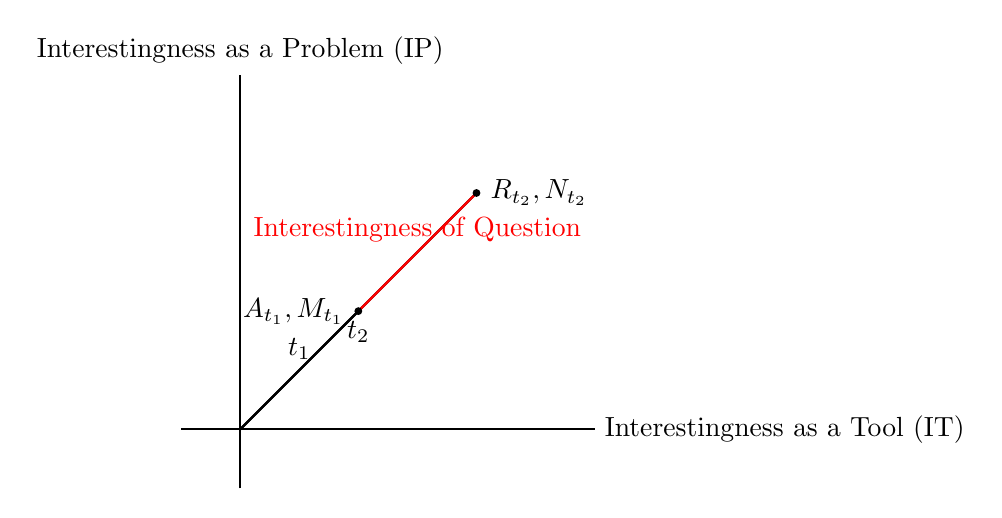
\begin{tikzpicture}[
    scale=1.5,
%    axis/.style={thick, ->, -latex', >=Stealth},
    axis/.style={thick},
%   vector/.style={thick, ->, -latex', >=Stealth, color=blue},
    vector/.style={thick},
    point/.style={circle, inner sep=1pt, fill, color=black}
]

% Coordinate axes
\draw[axis] (-0.5, 0) -- (3, 0) node[right] {Interestingness as a Tool (IT)};
\draw[axis] (0, -0.5) -- (0, 3) node[above] {Interestingness as a Problem (IP)};

% Points for t1 and t2
\coordinate (t1) at (1, 1);
\coordinate (t2) at (2, 2);

% Vectors for t1, t2, and the sum
\draw[vector] (0, 0) -- node[pos=0.5, above] {$t_1$} (t1);
\draw[vector] (0, 0) -- node[pos=0.5, below] {$t_2$} (t2);
\draw[vector, color=red] (t1) -- node[pos=0.5, above] {Interestingness of Question} (t2);

% Points and labels for t1 and t2
\node[point, label={left:$A_{t_1}, M_{t_1}$}] at (t1) {};
\node[point, label={right:$R_{t_2}, N_{t_2}$}] at (t2) {};

\end{tikzpicture}

In practice, we must calculate all possible combinations of topics with high interestingness as tools and those with high interestingness as problems. We then select the combinations with the highest interestingness as questions. Naturally, most questions generated using this approach will be meaningless, much like those arising during brainstorming sessions when researchers attempt to identify new tools for tackling difficult problems.

This methodology can be applied in other scenarios as well. For instance, a researcher familiar with problem $p$ might be interested in finding applicable tools to solve it. Similarly, a researcher specializing in tool $t$ may be interested in discovering open problems where his expertise can be applied.

The above procedure can be easily generalized to encompass multiple tools and possibly multiple problems. This leads to the application of two tools to a given problem ($ t_1 + t_2 \rightarrow p$), the application of a single tool to the combination of two problems ($t \rightarrow p_1 + p_2$), and so on. The exact meaning of these tool and problem combinations depends on the topics themselves and is left to the researcher's creative interpretation.

At times, it is beneficial to limit our search to specific areas of knowledge to identify interesting questions.

\begin{definition}\index{Intradisciplinary question} \index{Interdisciplinary question}
Let $\mathcal{A} \subset \mathcal{T}$ be a research area, and $t_1, t_2 \in \mathcal{T}$ be two topics. If both topics belongs to the same area, meaning $t_1, t_2 \in \mathcal{A}$, we say that the question $Q_{t_1 \rightarrow t_2}$ is \emph{intradisciplinary}, otherwise, we say that the question is \emph{interdisciplinary}.
\end{definition}

The most innovative questions tend to be interdisciplinary, as they have a lower likelihood of having been considered previously. This is because they require collaboration between specialists from different research areas. Interdisciplinary questions address our requirement \textbf{C1} for interesting questions, which dictates that the question must be new and original.

%
% Section: New Research Topics
%

\section{New Research Topics}
\label{sec:New_Research_Topics}

{\color{red} TODO: Review this section}

In the previous section our focus was in how to find new interesting research questions. In this section we will go one step beyond, and we will show how to identify new, previously unknown, research topics.

\begin{definition}\index{Unknown frontier}
In the two-dimensional space defined by relevance and nescience, the \textit{unknown frontier}, denoted by $\mathbb{F}$, is defined as the following arc:
\[
\mathbb{F} = \left\{(x,y) \mid x^{2}+y^{2}=max(\{N^2_{t} + R^2_{t}, t \in T'\}),x>0,y>0\right\} 
\]
\end{definition}

If we plot all the known research topics according to their relevance and nescience, the unknown frontier will cover them. Intuitively the \emph{unknown frontier} marks the frontier between what we do not know and we are aware that we do not know (we do not fully understand those topics), and what we do not known and we are not yet aware that we do not known those topics. This intuitive property is in general terms, since it may happen that some unknown topics lie under the unknown frontier as well.

\begin{definition}\index{New topics area}
Lets $T'$ the set of known research topics. The \emph{new topics area}, denoted by $\mathbb{S}$, is defined by:
\[
\mathbb{S} = \left\{(x,y) \mid x^{2}+y^{2}>max(\{N^2_{t} + R^2_{t}, t \in T'\}),x>0,y>0\right\} 
\]
\end{definition}

The new topics area contains all those unknown topics that we are not aware we do not know them (unknown unknown). The big issue is how to reach this new topics area if we do not know anything about the topics included in that area.

\begin{proposition}
\label{prop:new-topics-area}
Let $r \in T$ be a topic, if  $N^2_{r} + R^2_{r} > max(\{N^2_{t} + R^2_{t}, t \in T'\}$ then $t \in T \setminus T'$.
\end{proposition}
\begin{proof}
Let $N^2_{r} + R^2_{r} > max(\{N^2_{t} + R^2_{t}, t \in T'\}$ and suppose that $r \in T'$, then have that $max(\{N^2_{t} + R^2_{t}, t \in T'\}) \geq N^2_{r} + R^2_{r}$ that it is a contradiction, and so $t \in T \setminus T'$.
\end{proof}

Proposition \ref{prop:new-topics-area} together with the fact that the combined nescience of two topics is higher than the nescience of any of them isolated (Proposition {\color{red} XXX}), and that their combined relevance is higher that the relevance of any of them (Proposition \ref{prop:nondecreasing_relevance}), a possible approach to identify new topics could be by means of combining already existing interesting problems. In Figure \ref{fig:New-Topics} is depicted graphically the idea.

\begin{figure}[h]
\centering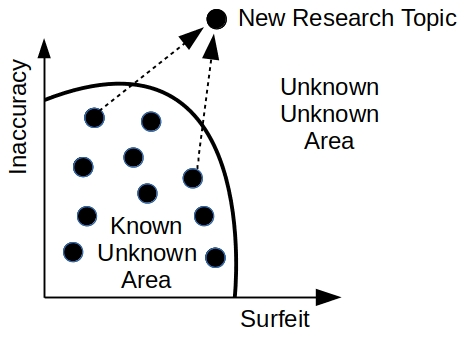
\includegraphics[scale=0.4]{NewTopics}
\caption{\label{fig:New-Topics}The discovery of new research topics}
\end{figure}

\begin{definition}\index{New topic}
Given two topics $t_{1}, t_{2} \in T'$, a \emph{new topic}, denoted by $S_{\left\{ t_{1},t_{2}\right\}}$, is the unordered pair $\left\{ t_{1},t_{2}\right\}$.
\end{definition}

The exact meaning of the new topic that results as the combination of topics $t_{1}$ and $t_{2}$ is left to the creative interpretation of the researcher.

\begin{definition}\index{Interestingness of a new topic}
The \emph{interestingness} of the new topic, denoted by $IS_{\left\{ t_{1},t_{2}\right\} }$, is given by:
\[
IS_{\left\{ t_{1},t_{2}\right\} } = R_{t_{1}}R_{t_{2}}+N_{t_{1}}N_{t_{2}}
\]
\end{definition}

In practice, what we have to do is to compute all possible combination of those topics with very large interestingness as problems $IP_{t}$ with themselves, and select the combinations with higher $IS$. Of course, some of the combinations generated would be totally meaningless. Advanced techniques from the area of natural language processing or machine learning could be used to try filter out those nonsense combinations.

\begin{definition}\index{Intradisciplinary new topic} \index{Interdisciplinary new topic}
Let $A \subset T$ a research area, and $t_{1}, t_{2} \in T$ two topics. If both topics belongs to the same area, that is $t_{1}, t_{2} \in A$, we say that the new topic $S_{\left\{ t_{1},t_{2}\right\} }$ is \emph{intradisciplinary}, otherwise, we say that the topic is \emph{interdisciplinary}.
\end{definition}

Again, the most innovative new topics would be by the combination of interdisciplinary topics, because the probability that somebody has already though about them is lower.

%
% Section: Classification of Research Areas
%

\section{Classification of Research Areas}

In the same way we studied the nescience of research areas (see Section \ref{sec:nescience_areas}), we could also study the interestingness of research areas.

\begin{definition}\index{Average interestingness of an area}
Given a research area $A\subset T$, we define the \emph{average interestingness
of the area as a source of interesting tools} by
\[
IT_{A}=\frac{1}{n}\sum_{t\in A}IT_{t}
\]
and the \emph{average interestingness of the area as a source of interesting
problems} by
\[
IP_{A}=\frac{1}{n}\sum_{t\in A}IP_{t}
\]
where $n$ is the cardinality of $A$.
\end{definition}

In this way we could compute the interestingness of mathematics, physics, biology, social sciences, and other disciplines as a source of interesting tools and problems. Other alternative measures of centrality and dispersion could be used for the characterization of research areas as well.

As I will show in Chapter \ref{chap:The-Scientific-Method}, the interestingness of mathematics as a source of tools is higher than the interest of social sciences, since mathematics is composed of topics with a high applicability that are very well understood, and that is not the case, in general, for social sciences. On the other hand, the interestingness of social sciences as a source of problems is higher than the interest of mathematics, since the topics studied by the social sciences are more relevant to humankind \footnote{Please mind that I am not saying that the topics addressed by mathematics are not relevant to humankind, what I am saying is that, in relative terms, the problems addressed by social sciences have a higher relevance.} and, in general, not very well understood.

\begin{example}\index{Areas in decay}
We could use the interestingness of an area to identify research areas in decay. A knowledge area is in decay (from the research point of view) if it has no enough interesting research problems. For example, although the aerodynamics of zeppelins is not fully understood (still some nescience), it is not longer useful (low relevance), since people does not use zeppelins to travel anymore, and so, the average interestingness is very low. Another example of area in decay is classical geometry: although it is relevant, our understanding of this subject is nearly perfect, since there are almost no unsolved problems, and so, its average nescience is very low. However, on the contrary to what happens in case of the aerodynamics of zeppelins, classical geometry is still very interesting as a source of tools.
\end{example}

It is worth to mention that we could add other metrics to provide a finer, or even alternative, characterization of the unknown unknown area. For example, we could add to nescience and relevance a third dimension with the probability that a topic description is true. However, these extended or alternative characterizations will be not considered in this book. Fortunately, the idea of how to reach the unknown unknown area is the same, regardless of the number and the metrics used (as long as these metrics satisfy some minimal mathematical properties, described in Chapters \ref{chap:Nescience} and \ref{chap:Interesting-Research-Questions}).

%
% References
%

\section*{References}

Popper and falsificationism

{\color{red} Review the following references}

\begin{itemize}

\item Freitas, A. A. (1999). On Objective Measures of Rule Surprisingness. In Proceedings of the Second European Symposium on Principles of Data Mining and Knowledge Discovery (PKDD '98), pp. 1-9.

\item Gureckis, T. M., \& Goldstone, R. L. (2009). How You Named Your Child: Understanding The Relationship Between Individual Decision Making and Collective Outcomes. Topics in Cognitive Science, 1(4), 651-674.

\item Klein, J. T. (1990). Interdisciplinarity: History, Theory, and Practice. Wayne State University Press.

\item Kuhn, T. S. (1962). The Structure of Scientific Revolutions. University of Chicago Press.

\item Newell, A., \& Simon, H. A. (1972). Human Problem Solving. Prentice-Hall.

\item Page, S. E. (2007). The Difference: How the Power of Diversity Creates Better Groups, Firms, Schools, and Societies. Princeton University Press.

\item Rescher, N. (1986). The Riddle of Existence: An Essay in Idealistic Metaphysics. University Press of America.

\item Schelling, T. C. (1978). Micromotives and Macrobehavior. W. W. Norton \& Company.

\end{itemize}
